\section{Inhibiting Superpositions with Activations}
\label{sec:act_fns}
The paper presents the activation function as a key in enabling the formation of superpositions due to their ability to 
filter out interference. As such, we demonstrate that modifying the activation can effectively control the model's usage of
superpositions. 
\newline
We propose ExReLU, a modified version of ReLU with a cut-off threshold of $t \in \mathbb{R}$, instead of $0$. By setting $t < 0$, its filtering effect for negative interference is weakened, thus
increasing the cost for the model to adopt superpositional representations.
\[
\text{ExReLU}(x) =
    \begin{cases}
        x & \text{if } x \geq t\\
        0 & \text{if } x < t
    \end{cases}
\] 

\subsection{Model}
We trained two sets of models, each with hidden layers of two neurons on a dataset with five features whilst varying the feature
sparsity. The first set used the normal ReLU activation, while the second used ExReLU with $t=-0.25$

\subsection{Results}
\begin{figure}[h]
	\centering
	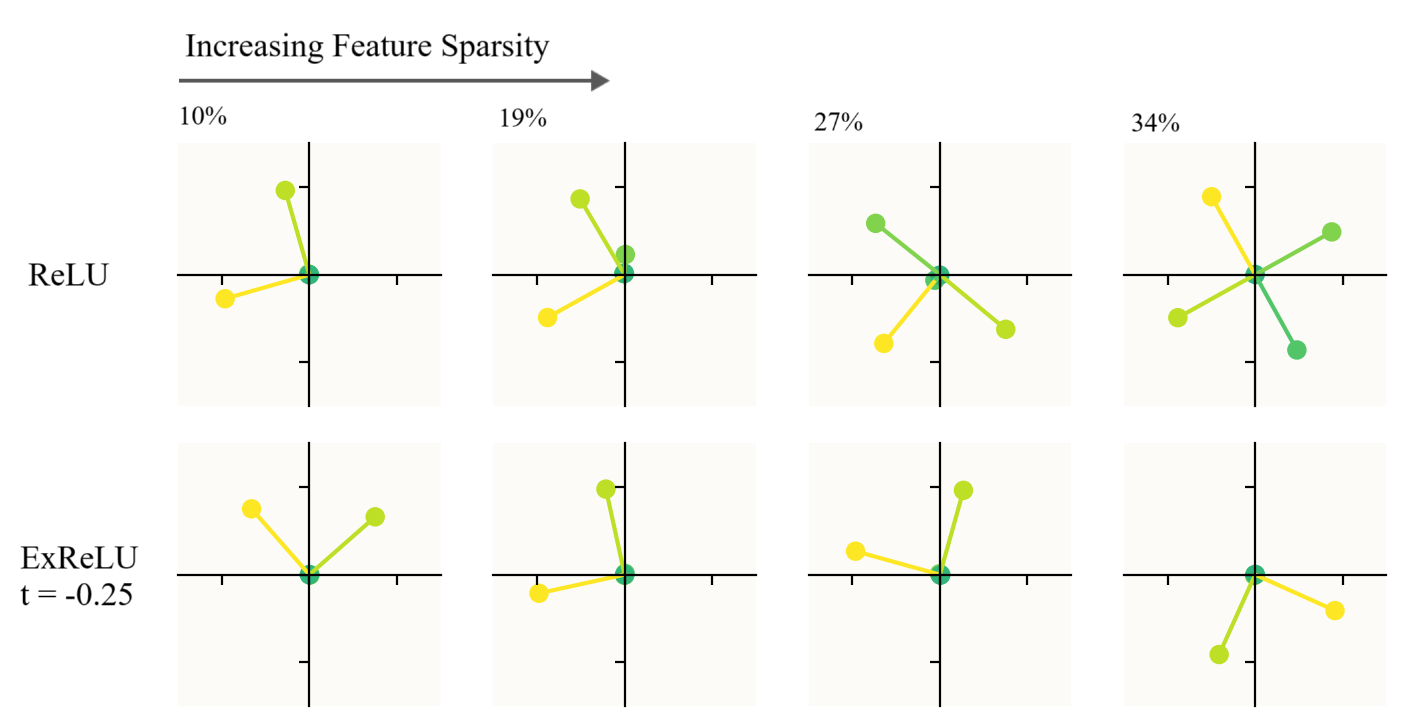
\includegraphics[width=1\linewidth]{figures/acts_diagram.png}
	\caption{Comparison of feature embeddings by the two model sets.}
	\label{fig:acts_diagram}
\end{figure}
Using the \href{https://colab.research.google.com/github/anthropics/toy-models-of-superposition/blob/main/toy_models.ipynb}{toy model framework} to visualize the hidden layer's representation of the features:
Figure \ref{fig:acts_diagram} shows that ExReLU has successfully suppressed the model's usage of superpositions in this instance.
